\section{Implementierung}
    \subsection{User Interface}
    
    	Zur Installation von \emph{kivy} unter Mac OS X wird auf der offiziellen Seite eine gepackte .app Datei angeboten. Wenn man sich diese genauer ansieht, enthält diese eine eigene \emph{Python}-Installation inklusive aller von \emph{kivy} benötigten Pakete. Allerdings kann man so seine \emph{Python}-Dateien nur mit dieser \emph{kivy App} ausführen. Ein versprochenes Shellscript, welches zumindest einen \texttt{kivy} Befehl für die Komandozeile bereitstellen soll, fehlt im Downloadverzeichnis. Es war auch nicht möglich diese Funktion von Hand mithilfe von Symlinks herzustellen.
        
        Auch abgesehen von diesen Problemen wäre es wünschenswert, \emph{kivy} in einer eigenen virtuellen \emph{Python}-Umgebung, erstellt von \texttt{virtualenv} über den Paketmanager \texttt{pip} zu installieren (???). Auf diese Weise können weitere für die Applikation benötigten Pakete auch in dieser Umgebung installiert werden.
        
        Das \emph{kivy} Framework bietet neben einem Eventsystem vor allem eine große Sammlung an User Interface Elementen und Layouts. Diese sind normale \emph{Python}-Klassen und können im Code instanziiert werden. Allerdings bietet \emph{kivy} auch eine eigene Syntax namens \emph{kv} (oder kivy-language) an, mithilfe welcher man die Layouts deskriptiv erstellen kann. Die Sprache erinnert ein wenig an eine Mischung aus dem \emph{CSS} Preprocessor \emph{Sass} und der \emph{HTML} Template Sprache \emph{Haml}.      
        
        \begin{figure}[H]
    		\centering
    		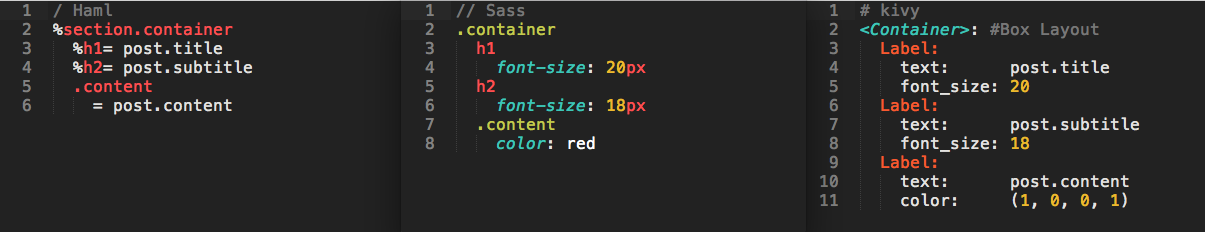
\includegraphics[width=15cm]{images/hamlsasskv.png}
    		\caption{Vergleich zwischen Haml Sass und kv}
    		\label{img:HamlSassKv}
		\end{figure}
        
        Man kann in \emph{kv} zwar auf \emph{Python}-Ausdrücke und Variablen zugreifen, aber alle Arten von Kontrollfluss  – wie z. B. Schleifen – stehen nicht zur Verfügung. So kann eine Liste von Buttons mit der Länge aller gefundenen Wortvorschläge nicht allein in \emph{kv} beschrieben werden. Als Lösung hierfür wurde in dieser Arbeit die Oberfläche in einzelne Module zerlegt. Jedes Modul hat eine eigene Klasse und dazu eine eigene \emph{kv} Datei. Die \emph{Python}-Klasse übernimmt so die Aufgabe eines Controllers, während die \emph{kv} Datei den View beschreibt. Allerdings werden immer noch viele Teile des Views im Controller instanziiert.
        
	\newpage
    \subsection{Wortschatz Verwaltung}
	\subsection{Kathegorisierung}
	\subsection{Wortvorhersage}
    \newpage